\documentclass[onecolumn]{IEEEtran}

\usepackage{amsmath, amsfonts, xspace, xcolor, url}
\usepackage{graphicx}
\usepackage{multicol}
\usepackage{lipsum}
\usepackage{hyperref}

\hypersetup{
colorlinks=true,       % false: boxed links; true: colored links
linkcolor=red,          % color of internal links (change box color with
%linkbordercolor)
citecolor=blue,       % color of links to bibliography
filecolor=magenta,   % color of file links
urlcolor=cyan           % color of external links
}

\IEEEaftertitletext{\vspace{-3\baselineskip}}

\begin{document}
\IEEEoverridecommandlockouts
% \IEEEpubid{\makebox[\columnwidth]{SE-HPCCSE16; Salt Lake City, Utah, USA; November 2016
% 978-1-5090-5224-0/16/\$31.00  \copyright
%         2014 IEEE \hfill} \hspace{\columnsep}\makebox[\columnwidth]{ }}
%
\IEEEpubid{\begin{minipage}{\textwidth}\ \\
\textcolor[gray]{0.5}{Proceeding: XX/\$XX.00 \copyright 20XX BRIC}
\end{minipage}}

\title{Sustainable Software via Generation}

% author names and affiliations
% use a multiple column layout for up to three different
% affiliations
\author{\IEEEauthorblockN{Spencer Smith, Jacques Carette\\}
\IEEEauthorblockA{\textit{Computing and Software Department, McMaster University, Canada}\\
Email: smiths@mcmaster.ca}
}

\maketitle

% \begin{abstract}
%   no abstract
% \end{abstract}

\renewcommand\IEEEkeywordsname{Keywords}

% \IEEEpeerreviewmaketitle
  
\begin{multicols}{2}
  
% \begin{IEEEkeywords}
% software documentation, generative programming, sustainable software
% \end{IEEEkeywords}
  
\textbf{\emph{Keywords---software documentation, generative programming, sustainable
    software}}
\medskip
% \section{Introduction} \label{SecIntroduction}

Sustainable software projects satisfy, for a reasonable amount of developer
effort, the requirements for the present, while also being maintainable,
reusable and reproducible to address future needs.  Achieving sustainability
requires documentation (requirements specification, design documents, test
plans, test reports, etc).  Developers recognize the value of documentation, but
often do not feel that they have the time/resources needed to write and maintain
it in the face of inevitable software changes
\cite{SmithJegatheesanAndKelly2016}.  A solution to this problem is to provide a
process that emphasizes documentation from the start, along with tools that
facilitate change.

\href{https://github.com/JacquesCarette/Drasil} {Drasil} provides such a process
and tools.  Drasil is a framework for generating all of the software artifacts
(code, documentation, scripts, etc.).  Drasil takes advantage of the inherent
knowledge duplication by capturing the knowledge once and providing means to
transform that information into all of the views needed within a given project.

Figure~\ref{Fig_DrasilAndChange} shows an example of the transformation of
captured knowledge (as shown in the darker bordered box at the top left).  The
software predicts whether a given plane of glass is likely to break when
subjected to an explosion.  An important property of the software is its name.
In this case the name is GlassBR.  In the generated artifacts the name GlassBR
appears more than 80 times -- in the folder structure, in the requirements
specification, in the README file, in the Makefile, and in the source code.  In
a conventional software project changing the name across all artifacts is
surprisingly difficult--difficult enough that the change may not be made.  With
Drasil a change like this is made by one change to the source knowledge and
regeneration.  By capturing domain knowledge, Drasil facilitates more than just
renaming.  For instance, if the assumption of a constant Load Distribution
Factor (LDF) changes, the regenerated software will have LDF as an input
variable.  Drasil also captures design decisions, like whether to log all
calculations, whether to in-line constants rather than show them symbolically,
etc. Drasil becomes even more powerful with the revelation that the same
knowledge can be reused in different projects.

Developers can now generate sustainable software, with documentation and code
that are consistent by construction.

%\lipsum[1-2]
\bibliographystyle{IEEEtran}
\bibliography{BRIC_2021}  
\end{multicols}

\begin{figure*}[h!]
\centering
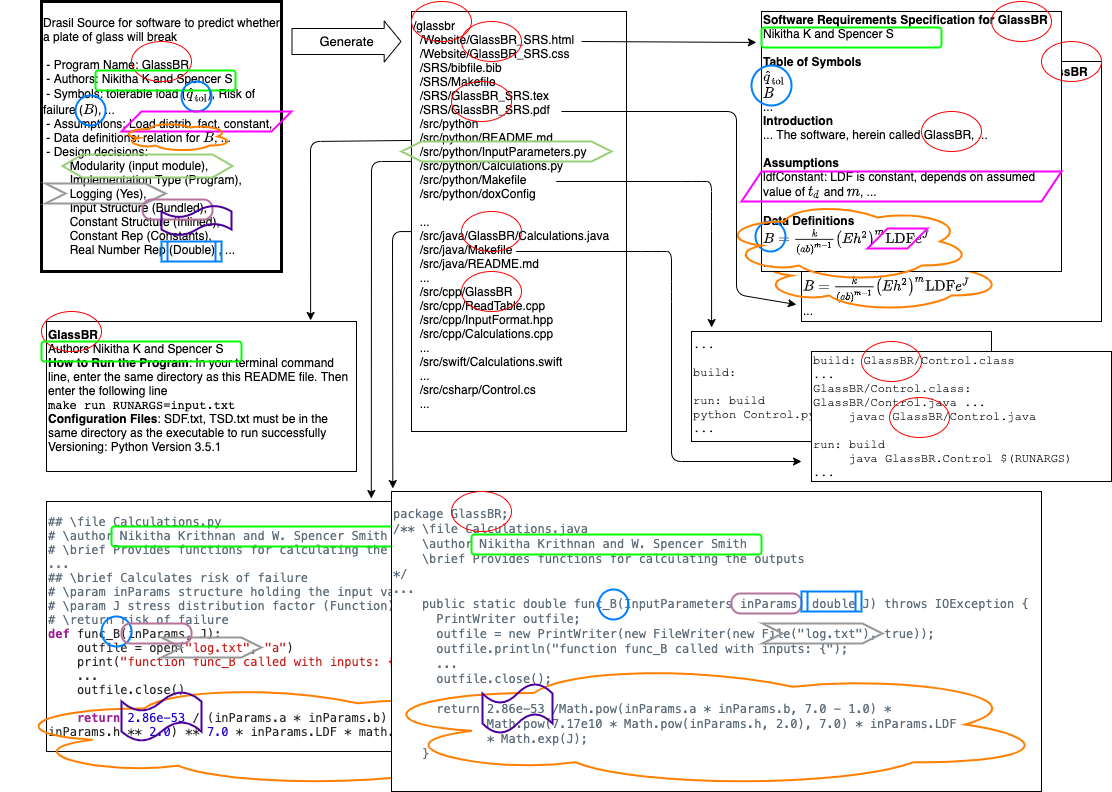
\includegraphics[width=0.7\textwidth]{./figures/DrasilSupportsChange.png}
\caption{Mapping between changes in Drasil source code to the generated
  artifacts.  The different colours and shapes show the connection between the
  source knowledge and the generated artifacts.}
\label{Fig_DrasilAndChange}
\end{figure*}

\end{document}
